% SVN info for this file
\svnidlong
{$HeadURL$}
{$LastChangedDate$}
{$LastChangedRevision$}
{$LastChangedBy$}

\chapter{Topologia quoziente}
\labelChapter{topologia quoziente}

\begin{introduction}
‘‘La visione topologica del mondo, rilassata e flessibile, mi metteva a mio agio. La Geometria classica mi sembrava invece moralista e conservatrice. Se la Geometria si veste con un completo, la Topologia indossa maglietta e jeans.''
\begin{flushright}
	\textsc{David S. Richeson,} sarto topologico.
\end{flushright}
\end{introduction}
\lettrine[findent=1pt, nindent=0pt]{R}{iprendiamo} l'\textit{oggetto elasticamente magico} con cui abbiamo introdotto il \autoref{chap:spazitopologici}: fra tutte le deformazioni che potevamo fare, \textit{incollare} parti di esso \textit{non} era consentito. E se invece provassimo a farlo? Quello che otterremo non è più uno spazio ‘‘\textit{equivalente}'' per un topologo a quello originale, ma comunque con molte proprietà interessanti da studiare.\\
La \textbf{topologia quoziente} formalizza questo concetto euristico di ‘‘incollare parti'' utilizzando le \textit{relazioni di equivalenza}; con il tipico approccio della Topologia Generale, faremo ciò dando delle semplici (seppur inizialmente poco intuitive) condizioni sulla continuità in modo da definire la topologia più adatta per l'\textit{insieme quoziente}.
\section{Topologia quoziente}
Accenniamo fin da subito che la situazione è \textit{duale} rispetto a quella dei sottospazi, analizzati nella sezione \ref{sottospazi}, pag. \pageref{sottospazi}.
\begin{define}[Topologia quoziente.]~{}\\
	Dato $X$ uno spazio topologico, $Y$ un \textit{insieme} e $\funz f X Y$ funzione suriettiva, la \textbf{topologia quoziente}\index{topologia!quoziente} su $Y$ indotta da $f$ è la topologia \textit{più fine} che rende $f$ continua.
\end{define}
Dalla definizione si ha che $\displaystyle A\subseteq Y \text{ aperto } \iff f^{-1}(A)\subseteq X$ aperto. Notiamo che l'implicazione $\Rightarrow)$ è necessaria affinché $f$ sia continua, mentre l'implicazione $\Leftarrow)$ è quella che caratterizza la topologia quoziente: infatti, se si considera un insieme $B\subseteq Y$ che non è aperto, allora la sua controimmagine $f^{-1}(B)\subseteq X$ non sarà aperta, altrimenti la topologia su $Y$ non sarebbe la più fine!
\begin{tips}
	Per verificare che un sottoinsieme sia aperto in $Y$ con la topologia quoziente bisogna verificare che la sua controimmagine è aperta.
\end{tips}
Vediamo ora un esempio che giustifica la terminologia ‘‘topologia quoziente''.
\begin{example}
	Sia $X$ uno spazio topologico e $\sim$ una relazione di equivalenza su $X$. Posto $Y=\nicefrac{X}{\sim}$ l'insieme quoziente e $\funztot \pi X Y x {\left[x\right]_\sim}$ la \textbf{proiezione al quoziente}\index{proiezione!al quoziente}, la topologia quoziente su $Y$ è quella che rende la proiezione continua.
\end{example}
Ricordiamo il primo Teorema fondamentale di isomorfismo per gli \textit{insiemi}, altresì chiamato \textit{decomposizione canonica}.
\begin{remember}~{}\\
	\begin{minipage}[t]{0.83\textwidth}
		Data una qualsiasi funzione suriettiva $\funz f X Y$ vi è la seguente relazione di equivalenza: 
		\begin{equation}
			\forall x,y\in X, \ x\sim y \iff f(x)=f(y)
		\end{equation}
		Inoltre, $\exists ! \funz h {\nicefrac{X}{\sim}} Y$ biunivoca tale che $f=h\circ\pi$, ponendo $h\left( [x] \right) \coloneqq f(x)$ in modo tale che il diagramma \textit{commuti}.
	\end{minipage}
	\begin{minipage}[t]{0.13\textwidth}\vspace{-10pt}
		\begin{tikzcd}
			X \arrow[r, "f"] \arrow[d, "\pi"']                                   & Y \\
			\nicefrac{X}{\sim} \arrow[ru, "\exists !h"', dotted] &
		\end{tikzcd}
	\end{minipage}
\end{remember}
Mostriamo che $h$ è ben definita e biunivoca.
	\begin{gather*}
		[x]=[y]\iff x\sim t\iff f(x)=f(y)\iff h([x])=h([y]) \implies h \text{ ben definita e iniettiva }\\
		f \text{ suriettiva } \implies h \text{ suriettiva}
	\end{gather*}
\subsection{Identificazione}
Tenendo a mente il concetto di immersione illustrato a pagina \pageref{immersione} illustriamo il concetto duale di \textit{identificazione}.
\begin{define}[Identificazione.]~{}\\
	Siano $X,Y$ spazi topologici e $\funz f X Y$ una funzione continua e suriettiva; $f$ si dice \textbf{identificazione}\index{identificazione} se $Y$ ha la topologia quoziente indotta da $f$.
\end{define}
In generale è difficile determinare quando una data funzione è un'identificazione, quindi ne cerchiamo una condizione \textit{sufficiente}.
\begin{theorema}[Funzione continua, suriettiva, chiusa/aperta è identificazione chiusa/aperta; Manetti, 5.4.]~{}\label{condizione sufficiente identificazione}\\
Sia $\funz f X Y$ continua, suriettiva e chiusa (o aperta), allora $f$ è un'identificazione chiusa (o aperta).
\end{theorema}
\begin{demonstration}
	Supponiamo che $f$ sia aperta. Dimostrare che è un'identificazione è equivalente al mostrare che $\displaystyle A\subseteq Y \text{ aperto } \iff f^{-1}(A)\subseteq X$ aperto.\\
	$\impliesdx$ Segue dalla continuità di $f$.\\
	$\impliessx$ Siccome $f$ è suriettiva allora vale $f(f^{-1}(A))=A$; essendo $f$ aperta segue che $A$ è aperto perché $f^{-1}(A)$ è aperto.
\end{demonstration}
Vediamo ora un esempio di identificazione chiusa e \textit{non} aperta.
\begin{example}
	Si consideri la funzione:
	\begin{equation*}
		\funztot f {[0, \ 2\pi]} {S^1} t {(\cos t, \ \sin t)}
	\end{equation*}
	È una funzione continua, suriettiva e chiusa (compatto in \textbf{Hausdorff}), dunque è un'identificazione chiusa. \\
	Tuttavia $f$ non è aperta: preso l'aperto $A=[0, \ 1)\subseteq [0, \ 2\pi]$, $f(A)$ non è aperto in $S^1$.
		\begin{center}
			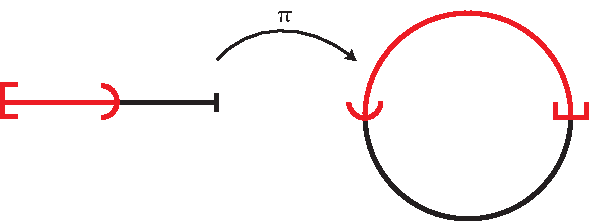
\includegraphics[trim=0cm 0cm 0cm 0cm,clip,scale=0.9]{images/half_circle-eps-converted-to.pdf}
		\end{center}
	\vspace{-6mm}
\end{example}
\begin{observe}
	Gli \textit{omeomorfismi} sono identificazioni chiuse e aperte.
\end{observe}
Che relazione c'è fra identificazioni ed quozienti dati da relazioni di equivalenza?
\begin{theorema}[Proprietà universale delle identificazioni; Manetti, 5.6.]~{}\\
\begin{minipage}[t]{0.83\textwidth}
		Dati $X,Y,Z$ spazi topologici, $g$ una qualsiasi funzione continua, $f$ identificazione con le mappe come in figura, allora:
		\begin{equation*}
			\exists! h \text{ continua } \colon g=h\circ f \iff \left( \forall x,y\in X, \ f(x)=f(y)\implies g(x)=g(y)  \right)
		\end{equation*}
	\vspace{-2mm}
		Cioè se e solo se $g$ è costante sulle fibre di $f$.
\end{minipage}
	\begin{minipage}[t]{0.13\textwidth}\vspace{-10pt}
		\begin{tikzcd}
			X \arrow[r, "g"] \arrow[d, "f"'] & Z \arrow[from=2-1, to=1-2, "\exists ! h"', dotted] \\
			Y  &
		\end{tikzcd}
	\end{minipage}
\end{theorema}
\begin{demonstration}
	Idealmente se $f$ fosse invertibile definiremmo $h=g\circ f^{-1}$. Tuttavia l'invertibilità di $f$ non è fra le ipotesi. Per ovviare a questo, utilizziamo la suriettività di $f$, considerando una controimmagine tramite $f$ e facendone l'immagine tramite $g$:
	\begin{equation*}
		y\in Y, \ h(y)\coloneqq g(x)\text{ con }x\in f^{-1}(y)
	\end{equation*}
	Con questa costruzione $h$ è ben definita siccome $g$ sarà costante sulle fibre di $f$. Verifichiamo che $h$ è continua tramite la definizione:
		\begin{gather*}
			U\subseteq Z \text{ aperto }, \ h^{-1}(U)\subseteq Y \iff f^{-1}(h^{-1}(U))\subseteq X \text{ aperto} \iff g^{-1}(U)\subseteq X \text{ aperto}
		\end{gather*}
	\vspace{-2mm}
	Siccome $g$ è continua allora lo è anche $h$.
\end{demonstration}
\begin{minipage}[t]{0.83\textwidth} \label{proprietà identificazione quoziente e mappa continua indotta}
Data allora $f$ continua, $\sim$ relazione di equivalenza e $\nicefrac{X}{\sim}$ spazio topologico con la topologia quoziente indotta dalla proiezione $\pi$, $\exists g$ continua $\iff \left( x\sim y \implies f(x)=f(y) \right)$, ovvero $f$ è costante sulle fibre di $\pi$.
\end{minipage}
\begin{minipage}[t]{0.16\textwidth}\vspace{-10pt}
 		\begin{tikzcd}
		 	X \arrow[r, "f"] \arrow[d, "\pi"']                                   & Y \\
 			\nicefrac{X}{\sim} \arrow[ur, "g"', dotted] &
		\end{tikzcd}
	\end{minipage}\\
\hspace{-1mm}
\begin{minipage}[t]{0.83\textwidth}\vspace{2mm}
In particolare, se $\sim$ è la relazione d'equivalenza indotta da $f$, e dunque si è nelle ipotesi del primo Teorema fondamentale di isomorfismo degli \textit{insiemi}, allora $\left( x\sim y \iff f(x)=f(y) \right) \implies \exists ! \overline{f}$ \textit{biettiva} e \textit{continua} tale che $f=\overline{f}\circ \pi$. Dunque vale:
	 	\end{minipage}
	\begin{minipage}[t]{0.16\textwidth}\vspace{-1pt}
			\begin{tikzcd}
				X \arrow[r, "f"] \arrow[d, "\pi"']                                   & Y \\
				\nicefrac{X}{\sim} \arrow[ur, "\overline{f}"', dotted] &
			\end{tikzcd}
	\end{minipage}\vspace{-1.5mm}\\
\begin{equation}
	\overline{f} \text{ omeomorfismo} \iff f \text{ identificazione}
\end{equation}
\vspace{-1.5mm}\noindent Riprendiamo l'esempio precedente ed esaminiamolo in termini di spazio quoziente.
\begin{example}~{$\nicefrac{D^n}{\sim}\cong S^n$}\\
	Consideriamo il caso $\mathbf{n=1}$:
	\begin{equation*}
		\funztot f {D^1=[0, \ 2\pi]} {S^1} t {(\cos t, \ \sin t)}
	\end{equation*}
	La funzione $f$ è un identificazione in quanto continua, suriettiva e chiusa (perché funzione da compatto in Hausdorff); pertanto $S^1\cong \nicefrac{[0, \ 2\pi]}{\sim}\cong \nicefrac{[0, \ 1]}{\sim}=\nicefrac{D^1}{\sim}$, con $\sim$ la relazione indotta da $f$:
	\begin{equation*}
		 s\sim t \iff \begin{cases}
			\cos s=\cos t \\
			\sin s =\sin t
		\end{cases} \iff s=t  \vee s=0,\ t=2\pi
	\end{equation*}
	Si può generalizzare in dimensione $n$ con l'identificazione:
	\begin{equation*}
		\funztot f {D^n} {S^n} {\mathbf{x}} {\left( 2\mathbf{x}\sqrt{1- \| \mathbf{x} \|^2}, \ 2\| \mathbf{x}\|^2 -1 \right)}
	\end{equation*}
	Dunque $\nicefrac{D^n}{\sim}\cong S^n$ per la relazione:
\begin{equation*}
	\mathbf{x}\sim \mathbf{y} \iff \mathbf{x}=\mathbf{y} \vee \labs \mathbf{x} \rabs ^2 = 1 = \| \mathbf{y} \| ^2
\end{equation*}
	In altre parole, ogni punto interno è \textit{in relazione con sé stesso} e tutti i punti sul bordo sono \textit{identificati} in un unica classe.
\end{example}
	
% LEZ 12
	\subsection{Quozienti tipici}
Vedremo ora degli esempi di spazi quoziente usati frequentemente.
\begin{intuit}
	Quando quozientiamo uno spazio topologico, possiamo immaginare che i punti contenuti nelle classi di equivalenza vengano ‘‘\textit{incollati}'' tutti in un unico punto per formare un nuovo spazio quoziente.\\
	Ad esempio, prendendo il disco $D^2$ con la relazione di equivalenza $\sim$ che identifica i punti del bordo:
	\begin{equation*}
		(x_1,\ y_1) \sim (x_2,\ y_2)\iff (x_1,\ y_1)=(x_2,\ y_2) \text{ oppure } x_1^2 +y_1^2= x_2^2 +y_2^2=1
	\end{equation*}
	I punti all'\textit{interno del disco} vengono tutti identificati in classi di equivalenza \textit{separate}, dunque passando allo spazio quoziente avremo una classe per \textit{ciascun} punto interno e un'\textit{unica} classe per tutti il bordo.\\
	Lo spazio quoziente ottenuto è $S^2$: possiamo ottenerlo visualmente ‘‘gonfiando'' l'interno del disco per poi chiudere il ‘‘palloncino'' ottenuto lungo i punti del bordo, come nella figura seguente.
	\begin{center}
		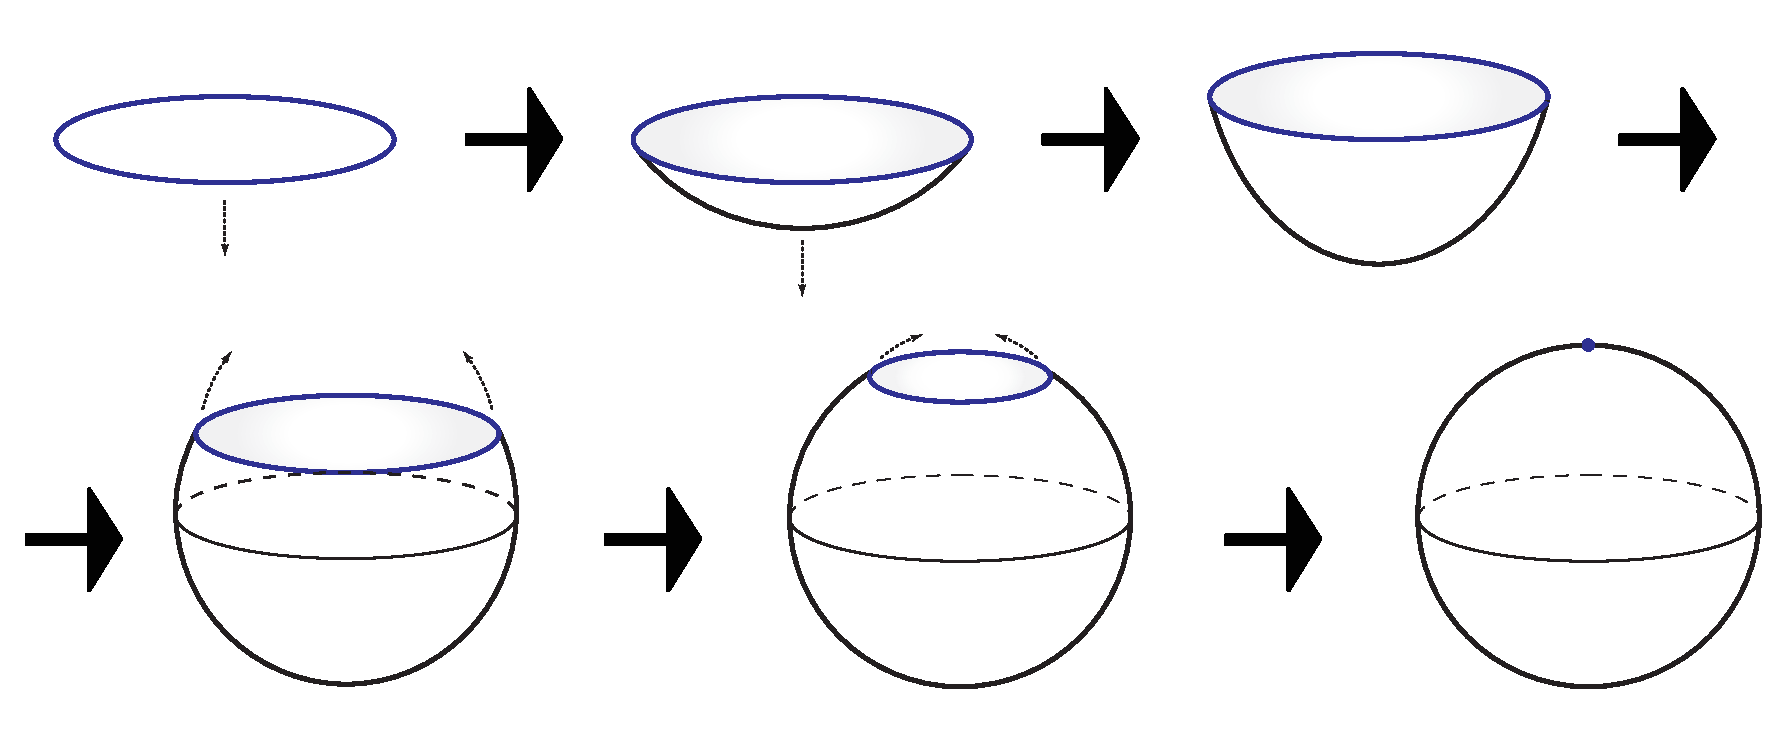
\includegraphics[trim=0cm 0cm 0cm 0cm,clip,scale=0.4]{images/disctosphere.pdf}
	\end{center}
\vspace{-6mm}
\end{intuit}
\subsubsection{Contrazione di un sottospazio ad un punto}
Sia $X$ uno spazio topologico, $A\subseteq X$, $\forall x,y\in X \ x\sim y\iff x=y$ oppure $x,y\in A$, ovvero ogni punto è in relazione con sé stesso e tutti i punti di $A$ sono in relazione fra loro, dunque quozientando si ‘‘\textbf{contraggono}''\index{contrazione} ad un unico punto.
\begin{example} $\nicefrac{D^n}{S^{n-1}}\cong S^n$ \\
	Cerchiamo ora di generalizzare l'esempio precedente. Ricordiamo che relazione c'è fra i dischi e le sfere:
		\begin{gather*}
			D^n=\text{ disco in } \realset^n=\{\mathbf{x}\in\realset^n \mid \labs \mathbf{x} \rabs \leq 1 \}\\
			S^{n-1}=\text{ bordo di } D^n=\{\mathbf{x}\in\realset^n \mid \labs \mathbf{x} \rabs = 1 \}
		\end{gather*}
	Considerando $\sim$ come la contrazione di $S^{n-1}$ ad un punto, si ha che $\nicefrac{D^n}{S^{n-1}} \cong S^n$.
\end{example}

\begin{attention}
	Anche se $X$ è di \textbf{Hausdorff} non è detto che $\nicefrac{X}{A}$ sia di \textbf{Hausdorff}!\\
	Se $A$ non è chiuso allora $\nicefrac{X}{A}$ non è neanche \textbf{T1}, infatti $\pi^{-1}([A])=A$ non chiuso implica che $[A]$ non lo è, quindi per la caratterizzazione degli spazi \textbf{T1} (definizione \ref{T1}, pag. \pageref{T1}) $\nicefrac{X}{A}$ non è \textbf{T1}.\\
	Tuttavia se $X$ è di \textbf{Hausdorff}, $K\subseteq X$ è compatto allora $\nicefrac{X}{K}$ è di \textbf{Hausdorff}. Nelle ‘‘Note aggiuntive'', a pag. \pageref{quozientehausdorffsuspaziocompatto}, si può trovare la dimostrazione di ciò.
\end{attention}
\subsubsection{Cono su uno spazio}
\begin{define}[Cilindro.]~{}\\
	Dato $X$ spazio topologico, si definisce \textbf{cilindro}\index{cilindro} su $X$ lo spazio $X\times \intv$.
\end{define}
\begin{define}[Cono.]~{}\\
	Il \textbf{cono}\index{cono} su $X$ spazio topologico è il quoziente $\displaystyle C\left(X\right)=\nicefrac{X\times\intv}{X\times\{1\}}$ oppure $\displaystyle C\left(X\right)=\nicefrac{X\times\intv}{X\times\{0\}}$.
\end{define}
\begin{intuit}
	Riprendiamo il procedimento intuitivo di incollare parti dello spazio originale per creare il quoziente per creare il \textit{cono} dal \textit{cilindro}: in questo caso, tutti i punti di una delle basi vengono incollati in uno.
\begin{center}
	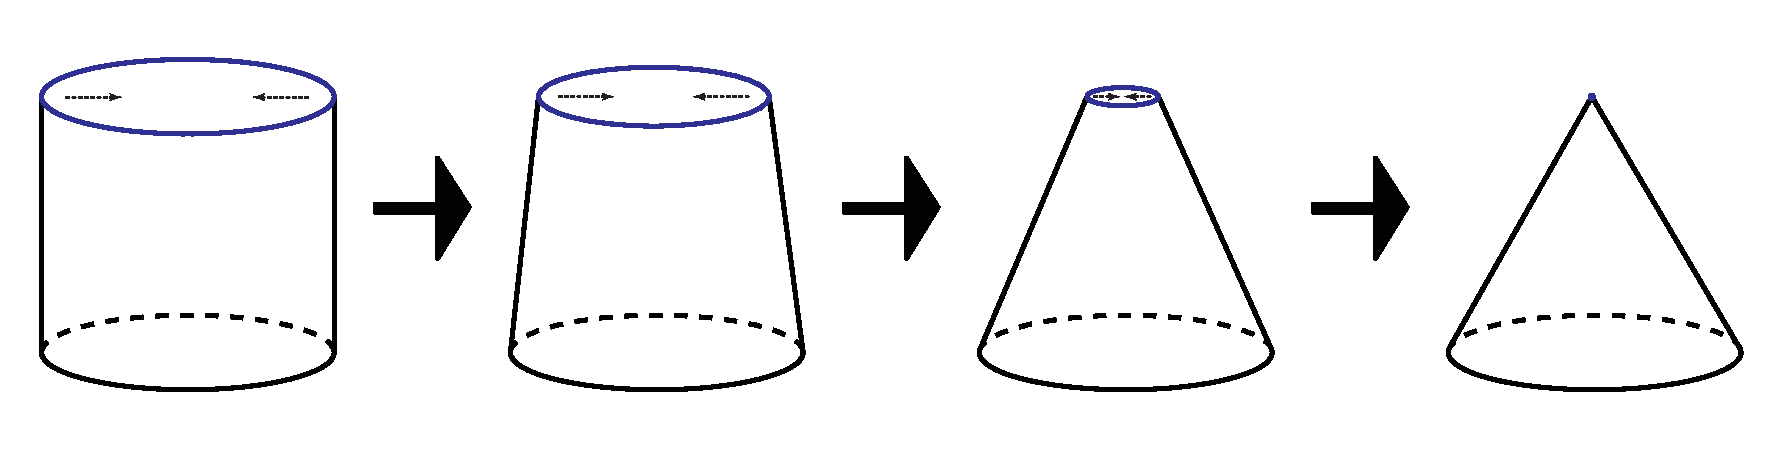
\includegraphics[trim=0cm 0cm 0cm 0cm,clip,scale=0.4]{images/cilindertocone.pdf}
\end{center}
\vspace{-6mm}
\end{intuit}
\begin{observe}
	Un cono è sempre c.p.a. rispetto al ‘‘vertice''.
\end{observe}
\begin{example} \textsc{Cono su} $S^n \cong D^{n+1}$.\\
	Studiamo i casi al variare della dimensione.\\
	$\mathbf{n=0)}$ $S^0=\{-1, \ 1\}=X \rightsquigarrow X\times\intv \rightsquigarrow \nicefrac{X\times\intv}{X\times \{0\}} \cong D^1$.
\begin{center}
	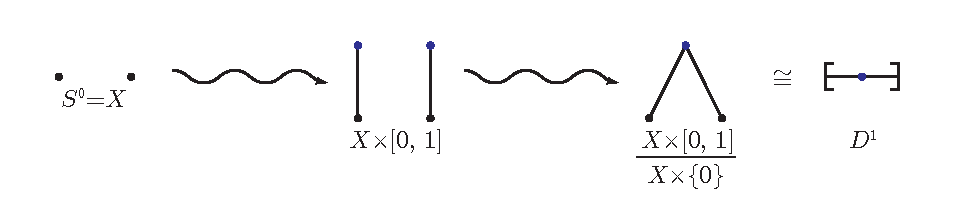
\includegraphics[trim=0cm 0cm 0cm 0cm,clip,scale=0.9]{images/cones0.pdf}
\end{center}
\vspace{-3mm}
	$\mathbf{n=1)}$ $S^1=X \rightsquigarrow X\times\intv \rightsquigarrow \nicefrac{X\times\intv}{X\times \{0\}} \cong D^2$.
\begin{center}
	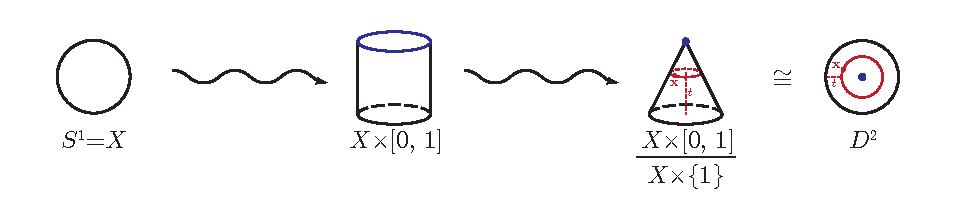
\includegraphics[trim=0cm 0cm 0cm 0cm,clip,scale=0.9]{images/cones1.pdf}
\end{center}
\vspace{-3mm}
	In generale, considerata la funzione:
	\begin{equation*}
		\funztot f {S^n\times\intv} {D^{n+1}} {(\mathbf{x}, \ t)} {t\mathbf{x}}
	\end{equation*}
\begin{minipage}[t]{0.72\textwidth}
	Essa è continua, suriettiva, chiusa (compatto in \textbf{Hausdorff}), dunque $f$ è identificazione e induce l'omeomorfismo $\overline{f}$ tra il cono $C\left(S^n\right)$ e il disco $D^{n+1}$.
Verifichiamo che la relazione di equivalenza indotta da $f$ è proprio quella di contrazione:
\end{minipage}
\begin{minipage}[t]{0.29\textwidth}\vspace{-10pt}
	\begin{tikzcd}
		{S^{n}\times[0,\ 1]} & {D^{n+1}} \\
		{C\left(X\right)}
		\arrow["f", from=1-1, to=1-2]
		\arrow["\pi"', from=1-1, to=2-1]
		\arrow["{\overline{f}}"', from=2-1, to=1-2]
	\end{tikzcd}
\end{minipage}
		\begin{gather*}
			(\mathbf{x}, \ t)\sim (\mathbf{y}, \ s) \iff f(\mathbf{x}, \ t)=f(\mathbf{y}, \ s) \iff t\mathbf{x}=s\mathbf{y} \iff \begin{cases}
				\mathbf{x=y}, \ t=s \\
				t=s=0
			\end{cases}\\
			\text{Se } t\neq 0 \implies \mathbf{x}=\frac{s}{t}\mathbf{y}, \text{ ma } \labs\mathbf{x}\rabs=1 \implies \left| \frac{s}{t} \right| \underbrace{\labs\mathbf{y}\rabs}_{=1}=1 \implies \left| \frac{s}{t} \right| =1 \implies s=t \implies \mathbf{x=y}
		\end{gather*}
	\vspace{-6mm}
\end{example}
\subsubsection{Retta con 2 origini} \label{retta 2 origini}
Analizziamo un particolare spazio topologico che spesso funge da controesempio (ad esempio per le varietà topologiche, sez. \ref{retta2originivarietà}, pag. \pageref{retta2originivarietà}): \textbf{la retta con 2 origini}. \\
Sia $X=\realset\times\{a,b\}$.
\begin{center}
	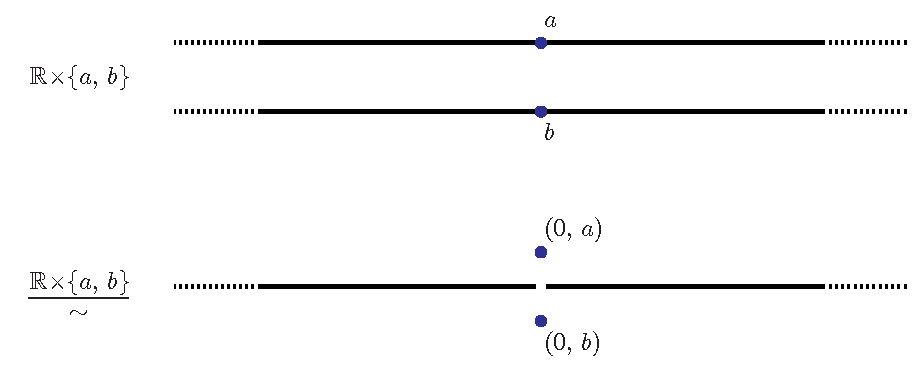
\includegraphics[trim=0cm 0cm 0cm 0cm,clip,scale=0.95]{images/line2origins.pdf}
\end{center}
Vogliamo definire una relazione di equivalenza che lasci ‘‘separate'' solo le origini:
	\begin{gather*}
		(x, \ \alpha)\sim (y, \ \beta) \iff
			\begin{cases}
				x=y,\ \alpha=\beta \\
				x=y\neq 0
			\end{cases}		
	\end{gather*}
\textsc{Proprietà}:
\begin{enumerate}
	\item $Y\coloneqq \nicefrac{X}{\sim}$ è c.p.a., infatti se i punti $[(x, \ \alpha)]$ e $[(y, \ \beta)]$ sono tali che $x\neq 0 \neq y$ basta prendere il segmento $\overline{xy}$ sulla retta $\realset\times\{a\}$ e proiettarlo. Per unire $[(0,\ a)]$ e $[(0, \ b)]$ basta unire entrambi con un cammino al punto $[(1, \ a)]=[(1, \ b)]$
	\item $Y$ non è di \textbf{Hausdorff}: tutti gli intorni di $[(0, \ a)]$ si intersecano con tutti gli intorni di $[(0, \ b)]$.
	\item $Y$ è \textit{localmente omeomorfo} a $\realset$, infatti ogni punto ha un intorno omeomorfo ad un intervallo aperto di $\realset$
	\item $\exists K_1, \ K_2\subseteq Y$ compatti tali per cui $K_1\cap K_2$ \textit{non} è compatto: basta prendere $K_1=\pi\left([-1, \ 1]\times \{a\} \right)$ e $K_2=\pi\left([-1, \ 1]\times \{b\} \right)$ compatti in $Y$, ma $K_2\cap K_2= [-1,\ 0) \cup (0,\ 1]$ \textit{non} è compatto in $Y$.
\end{enumerate}
\subsection{Quoziente di Hausdorff}
Cerchiamo ora delle condizioni per avere un \textit{quoziente di} \textbf{Hausdorff}.
\begin{theorema}[Condizioni sufficienti per il quoziente di Hausdorff.]~{}\label{quozientehausdorff}\\
Sia $\funz f X Y$ continua e identificazione con $X$ compatto e di \textbf{Hausdorff}, allora sono equivalenti:
		\begin{enumerate}
			\item $Y$ è di \textbf{Hausdorff}.
			\item $f$ chiusa.
			\item $K=\left\{ (x_1,\ x_2)\in X\times X \mid f(x_1)=f(x_2) \right\}$ chiuso in $X\times X$.
		\end{enumerate}
	\vspace{-3mm}
\end{theorema}
\begin{demonstration}~{}\\
	$1 \implies 3)$  Poichè $Y$ è di \textbf{Hausdorff}, per il teorema \ref{hausdorff diagonale chiusa}, pag. \pageref{hausdorff diagonale chiusa}, la diagonale $\Delta_Y$ è chiusa. Si consideri ora la seguente funzione:
	\begin{equation*}
		\funztot {h\coloneqq f\times f} {X\times X} {Y\times Y} {(x_1,\ x_2)} {\left( f(x_1), \ f(x_2) \right) }
	\end{equation*}
	Essa è continua perché lo è $f$. Notiamo che $K=h^{-1}(\Delta_Y)$; allora $K$ è chiuso in quanto controimmagine della diagonale, chiusa per ipotesi di Hausdorff.
	\[\begin{tikzcd}
		X &&&& Y \\
		& {X\times X} && {Y\times Y} \\
		X &&&& Y
		\arrow["{h\coloneqq f\times f}", from=2-2, to=2-4]
		\arrow["{p_1}"', from=2-2, to=1-1]
		\arrow["{p_2}", two heads, from=2-2, to=3-1]
		\arrow["{q_2}"', two heads, from=2-4, to=3-5]
		\arrow["{q_1}", two heads, from=2-4, to=1-5]
		\arrow["f"', from=3-1, to=3-5]
		\arrow["f", from=1-1, to=1-5]
	\end{tikzcd}\]
	$3\implies 2)$ Per dimostrare che $f$ è chiusa bisogna far vedere che $\forall C\subseteq X$ chiuso $f(C)\subseteq Y$ è chiuso; $Y$ ha la topologia quoziente perché $f$ è identificazione, quindi dobbiamo mostrare che $f^{-1}\left( f(C) \right)\subseteq X$ sia chiuso. Notiamo che $f^{-1}\left( f(C) \right)= p_1(K\cap p_2^{-1}(C))$:
	\begin{equation*}
		\begin{array}{ll}
		p_2^{-1}(C)=X\times C & \implies
		\begin{array}{ll}
			K\cap p_2^{-1}(C) & = \left\{ (x_1,\ x_2)\in X\times X \mid f(x_1)=f(x_2)\in f\left(C\right) \right\}\\
			& = \left\{ (x_1,\ x_2)\in X\times X \mid x_1\in f^{-1}\left(f\left(C\right)\right) \right\}
		\end{array}\\
		p_1(K\cap p_2^{-1}(C)) & = \left\{ (x_1,\ x_2)\in X\times X \mid x_1\in f^{-1}\left(f\left(C\right)\right) \right\}=f^{-1}\left( f(C) \right)
	\end{array}
	\end{equation*}
	Si conclude dunque che $f$ è chiusa in base alle proprietà delle proiezioni $p_1$ e $p_2$:
		\begin{equation*}
			\begin{array}{ll}
				p_2 \text{ continua e $C$ chiuso } & \implies p_2^{-1}(C) \text{ chiuso} \\
				K \text{ chiuso } &\implies p_2^{-1}(C)\cap K \text{ chiuso}\\
				X \text{ compatto} & \implies p_1 \text{ chiuso}\implies p_1 \left( K\cap p_2^{-1}(C) \right)=f^{-1}\left( f(C)\right) \text{ chiuso}
			\end{array}
		\end{equation*}
	$2\implies 1)$ Serve il \textit{teorema di Wallace}, pertanto non ne affronteremo la dimostrazione.
\end{demonstration}
\begin{observe}
	Nella dimostrazione $1\implies 3)$ \textit{non} si è utilizzato che $f$ è un'identificazione, dunque vale \textit{in generale}!
\end{observe}
